\section{Full Sheaf Cobordism}
Suppose we have a positive braid word $\omega = s_{i_1}\cdots s_{i_k}$ on $n$ strands, then we have an embedding of the cylindrical closures of $\omega$ and the trivial braid $\omega_{\emptyset}$ in a Riemann sphere with punctures at $0,\infty$ described in section ??. Suppose we have an alternating sheaf on the natural alternating diagram associated to $\omega \coprod \omega_\emptyset$ when restricted to the $j^{th}$ generator region is described by the following legible diagram
\begin{figure}[H]
    \centering
    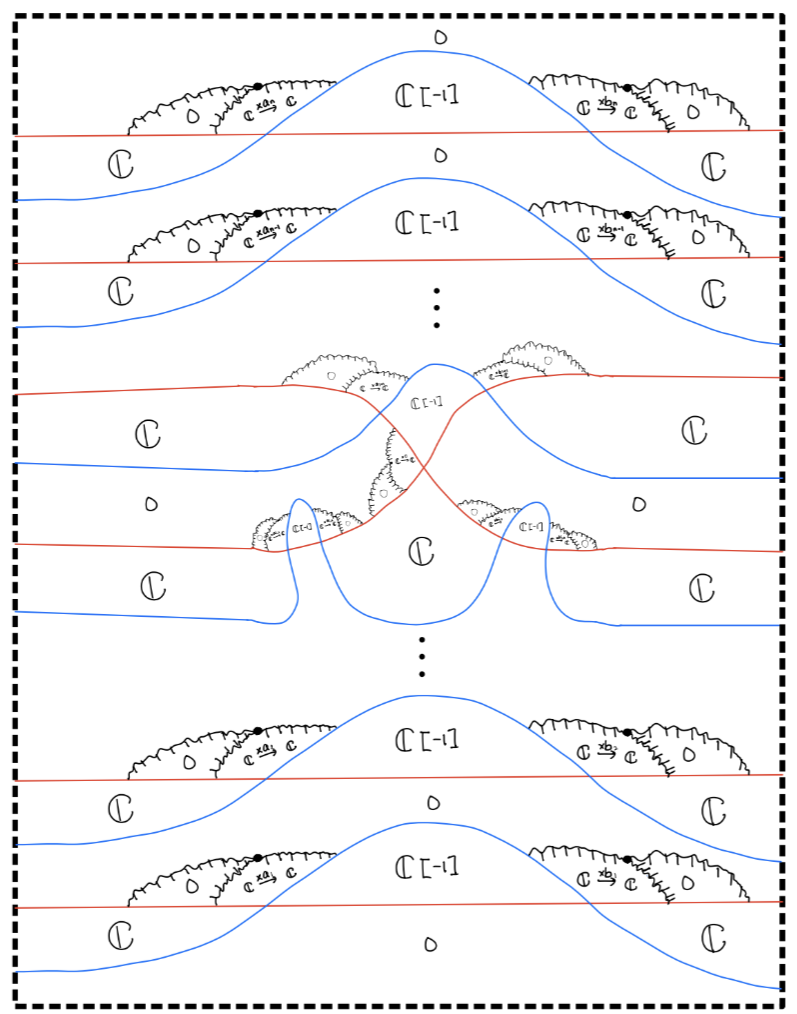
\includegraphics[scale = 0.95]{diagrams/cobord_full/1.png}
    \caption{}
    \label{fig:your-label}
\end{figure}
and when restricted to inter-generator regions is described by the following squiggly legible diagram
\begin{figure}[H]
    \centering
    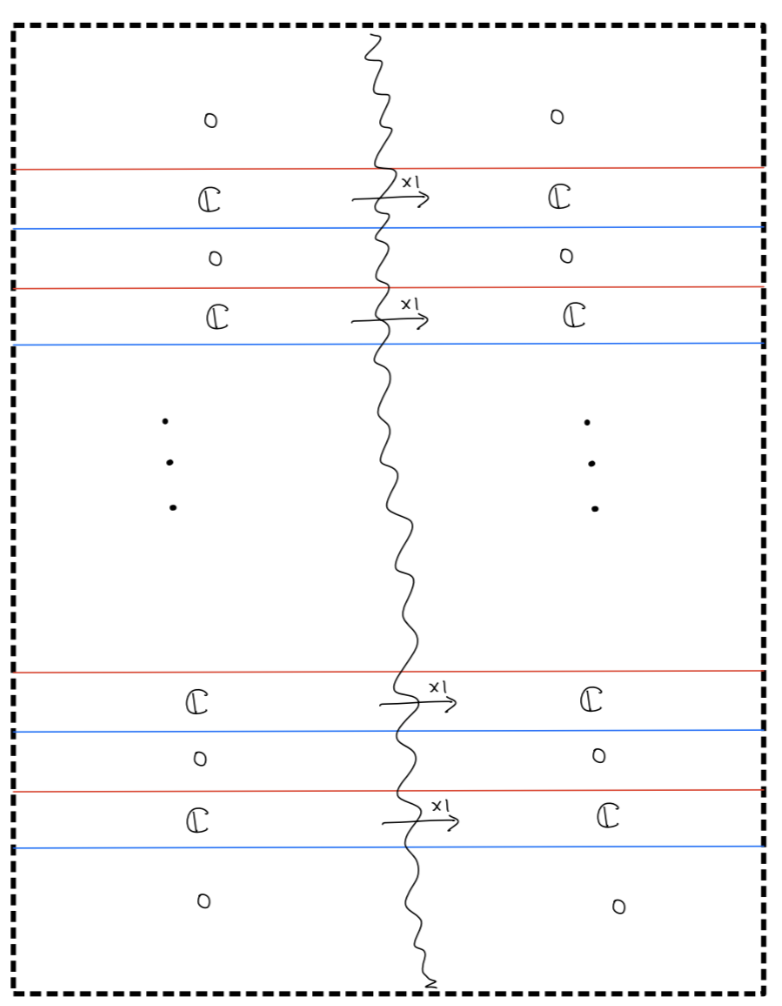
\includegraphics[scale = 0.95]{diagrams/cobord_full/2.png}
    \caption{}
    \label{fig:your-label}
\end{figure}
then we define a sheaf cobordism from the above alternating sheaf whose underlying Legendrian isotopy and at the separated diagram of $\omega \coprod \omega_\emptyset$, thereby describing a cluster coordinate.

\begin{enumerate}[label = (Step \arabic*)]
\item to the $j^{th}$ generator regions($j=1,\cdots,k$), apply $cobord_{gen(n)}$, we get on the $j^{th}$ generator region
\begin{figure}[H]
    \centering
    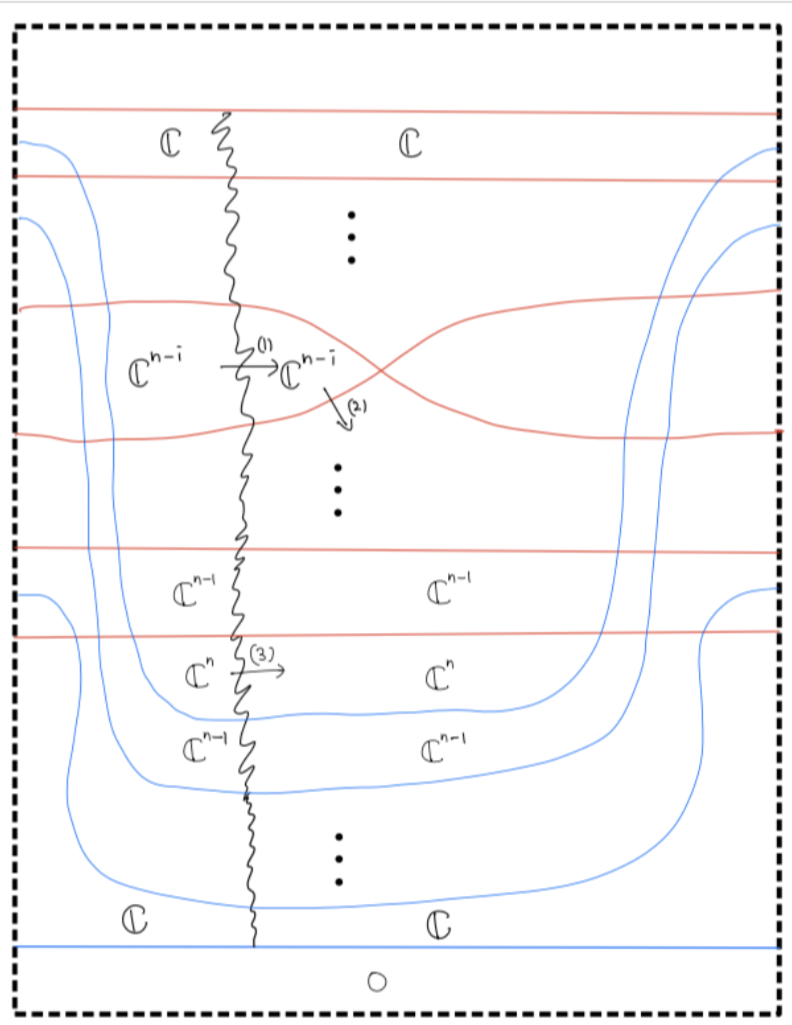
\includegraphics[scale = 0.95]{diagrams/cobord_full/3.png}
    \caption{}
    \label{fig:your-label}
\end{figure}
\textbf{Generization maps}
\begin{enumerate}
\item $diag(d^j_n,\cdots, d^j_{i+1})$
\item $\iota_0 \circ diag(1,\cdots, 1) + e'I_{n-i+1,n-i}$
\item $diag(d^j_n,\cdots, d^j_{1})+ eI_{n-i+1,n-i}$
\end{enumerate}
where
\begin{itemize}
\item $a_i=a_{i,1}a_{i,2}^{-1}$ and $b_i=b_{i,1}^{-1}b_{i,2}$
\item $d_r = a_rb_r^{-1}$
\item $e = -a_{i+1}b_i^{-1}c$
\item $e' = d_{i+1}^{-1}e$
\end{itemize}

and on the inter-generator regions we get
\begin{figure}[H]
    \centering
    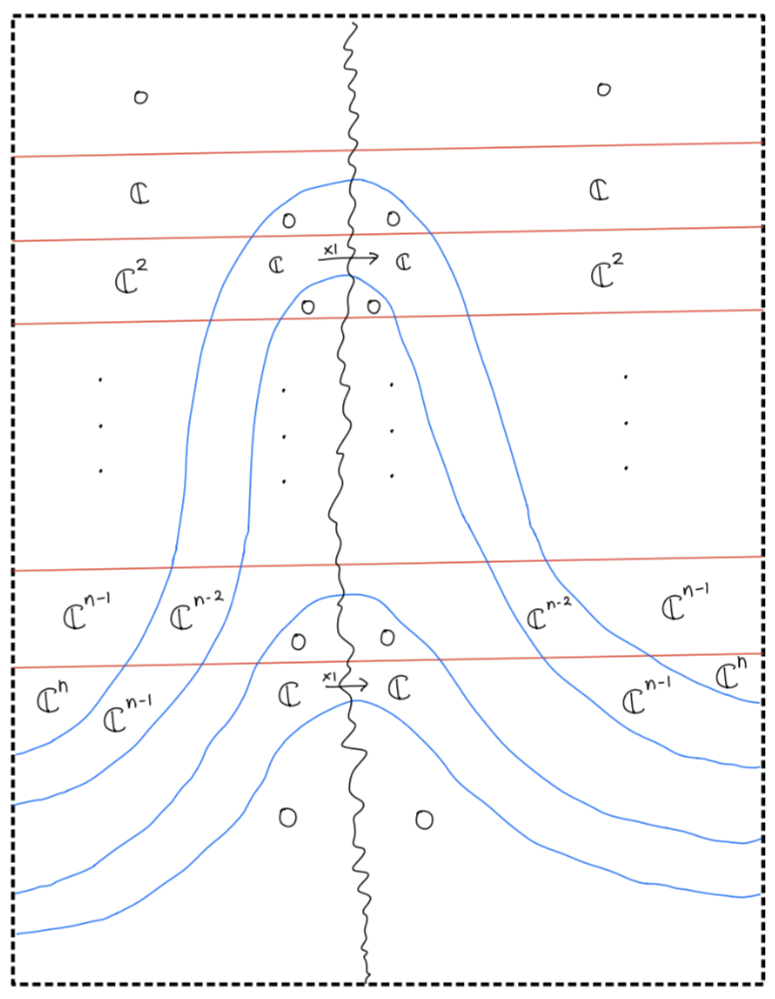
\includegraphics[scale = 0.95]{diagrams/cobord_full/4.png}
    \caption{}
    \label{fig:your-label}
\end{figure}
\item to the inter-generator regions, we apply $cobord_{inter}(n)$, on the $j^{th}$ generator region, we get
\begin{figure}[H]
    \centering
    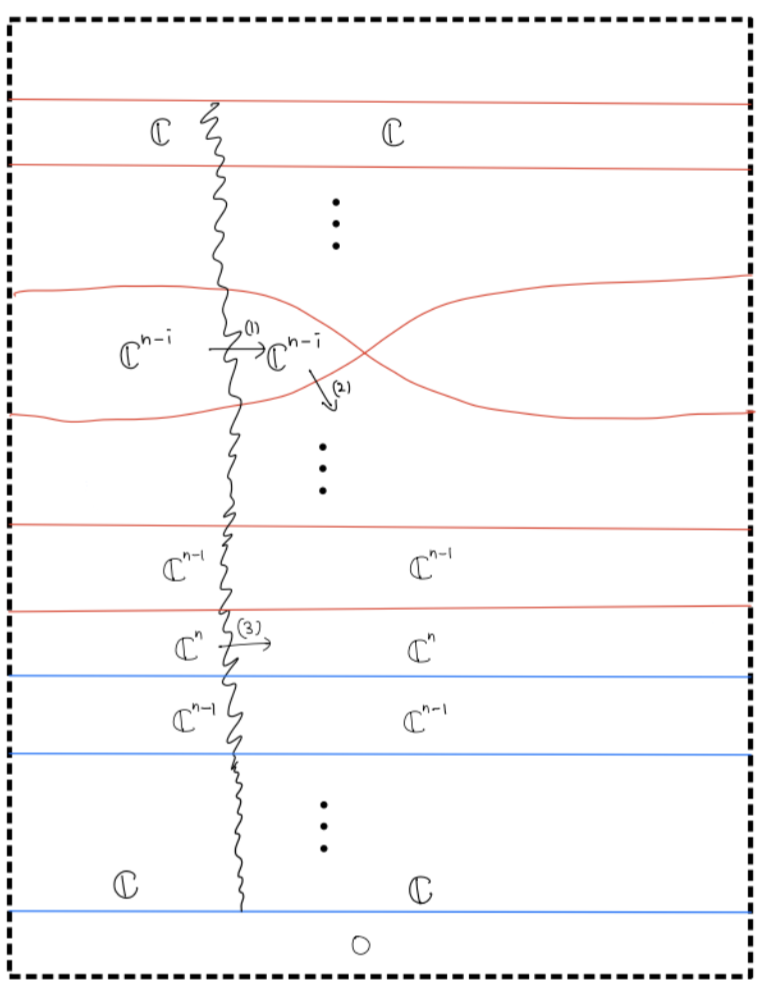
\includegraphics[scale = 0.95]{diagrams/cobord_full/5.png}
    \caption{}
    \label{fig:your-label}
\end{figure}
\textbf{Generization maps}
\begin{enumerate}
\item $diag(d^j_n,\cdots, d^j_{i+1})$
\item $\iota_0 \circ diag(1,\cdots, 1) + e'I_{n-i+1,n-i}$
\item $diag(d^j_n,\cdots, d^j_{1})+ eI_{n-i+1,n-i}$
\end{enumerate}
and on the inter-generator regions, we get
\begin{figure}[H]
    \centering
    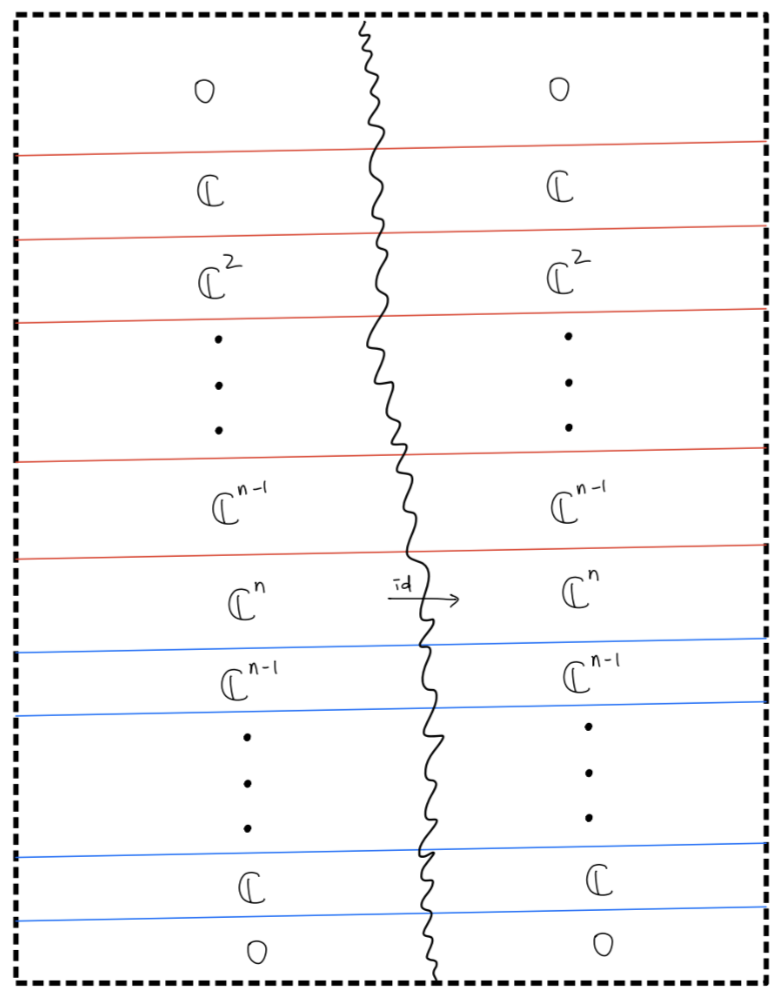
\includegraphics[scale = 0.95]{diagrams/cobord_full/6.png}
    \caption{}
    \label{fig:your-label}
\end{figure}
\end{enumerate}